% new_TLP2egui.tex / guide for TLP
% v2.12, released 23-apr-2003
%   (based on JFP2egui.tex v1.01) and tlp2egui.tex
% Copyright (C) 2000,2001,2002,2003, 2012 Cambridge University Press

\NeedsTeXFormat{LaTeX2e}

\documentclass{new_tlp}

%\usepackage[sort&compress,square,comma,authoryear]{natbib}
%\bibliographystyle{plainnat}
%\bibliographystyle{amsalpha}
\bibliographystyle{acmtrans}

\usepackage[toc,page]{appendix}
\usepackage{url}
\usepackage{mathptmx}
\usepackage{graphicx}
\usepackage{subfigure}
%%% Macros for the guide only %%%
\hyphenation{either}
\providecommand\AMSLaTeX{AMS\,\LaTeX}
\newcommand\eg{\emph{e.g.}\ }
\newcommand\etc{\emph{etc.}}
\newcommand\bcmdtab{\noindent\bgroup\tabcolsep=0pt%
  \begin{tabular}{@{}p{10pc}@{}p{20pc}@{}}}
\newcommand\ecmdtab{\end{tabular}\egroup}
\newcommand\rch[1]{$\longrightarrow\rlap{$#1$}$\hspace{1em}}
\newcommand\lra{\ensuremath{\quad\longrightarrow\quad}}

  \title[Theory and Practice of Logic Programming]
        {Encoding Selection for Solving Hamiltonian Cycle Problems with ASP}

\author[Liu Liu and Mirek Truszczynki]
 {LIU LIU and MIREK TRUSZCZYNSKI\\
 University of Kentucky, Lextington, KY, USA\\
 \email{liu.liu@uky.edu and mirek@uky.edu}}

%\jdate{March 2003}
%\pubyear{2003}
\pagerange{\pageref{firstpage}--\pageref{lastpage}}
%\doi{S1471068401001193}

\newtheorem{lemma}{Lemma}[section]

\begin{document}
\nocite{*}% includes all entries of BibTeX database into the list of references.


\label{firstpage}

\maketitle

  \begin{abstract}
It is common for search and optimization problems to have alternative equivalent encodings in ASP. 
Which of these encodings lends itself best to ASP solvers is 
difficult to answer as typically no encoding is uniformly better 
than others when evaluated on broad classes of problem instances.
We posit that one can improve the solving ability of ASP by using machine 
learning techniques to select encodings likely to perform well on 
a given instance. In this paper, we show the viability of this approach by 
studying the hamiltonian cycle problem. We propose several equivalent 
encodings of the problem and several classes of hard instances. We build models to 
predict the behavior of each encoding based on their performance history, 
and then show that by selecting encodings for a given instance 
using the learned performance predictors leads to significant performance gains.
    
  \end{abstract}

  \begin{keywords}
    Encoding Selection, Machine Learning, Answer Set Programming
  \end{keywords}

%\tableofcontents

\section{Introduction}
Answer Set Programming (ASP) is a declarative formalism for solving difficult 
search and optimization problems whose decision versions belong to the 
class $\Sigma_2^P$ \cite{BrewkaET11}. Problems are modeled in ASP by answer 
set programs; instances to a problem are modeled by sets of ground atoms. 
A program for a problem is designed so that when combined with ground atoms 
describing an instance, it yields a program whose answer sets represent
solutions to the problem for that instance \cite{mt99}. A consequence of this
approach is that to solve problems with ASP, one needs tools that compute 
answer sets of programs. Several such tools, commonly referred to as 
\emph{solvers}, have been proposed. Most notable among them are \textit{dlv} 
\cite{LeonePFEGPS06},\footnote{\url{http://www.dlvsystem.com}.} 
\textit{gringo/clasp}~\cite{potsdamBook}\footnote{\url{https://potassco.org.}} 
and \textit{wasp} \cite{AlvianoDFLR13}.\footnote{\url{http://alviano.github.io/wasp/.}} 
These tools have been shown to be especially effective on search and 
optimization problems whose decision versions are in the class NP, including 
many problems of practical interest \cite{GebserMR17,ErdemGL16}. 

Despite the ease of modeling and the demonstrated potential of ASP, using it is 
not without challenges. First, it is unlikely a single solver will emerge
that would uniformly outperform all others. Second, solvers commonly come
with tens, even hundreds, of parameters. The ability to choose the right 
solver and the right parameter configuration on the \emph{per-instance} 
basis may then be the difference between solving a problem within an acceptable 
time bound or having a solver (even an excellent one) run ``forever.'' 
%This issue has long been recognized by the research community. 
Consequently, 
solver selection, portfolio solving, and automated parameter configuration 
have all been extensively studied in ASP \cite{MarateaPR14,HoosLS14}, as well as 
in other fields \cite{Rice76,KerschkeHNT19}. The key idea is to learn
instance-driven performance models and use them, given an instance, to
select a solver (or a parameter configuration) that might perform well
on that instance. 
This research has resulted in significant performance enhancements for ASP. 

However, there is yet another possibility for enhancing the effectiveness 
of ASP. It is well known that problems have alternative equivalent encodings 
as answer set programs and these encodings typicaly perform differently when 
run on different instances. Consequently, two possible lines of attack emerge: 
(1) to establish program rewriting heuristics to generate better performing 
programs, and (2) to develop methods for encoding selection and encoding 
portfolio solving, similar to those used in algorithm selection and 
portfolio solving~\cite{GomesS01,HoosLS14}. The first idea has received some 
attention in recent years \cite{BuddenhagenL15,BichlerMW16,HippenL19}. 
However, the approach to capitalize on the availability of collections of 
equivalent encodings, produced ``by hand'' or generated automatically from 
a ``hand-made'' one, has not yet been explored.

We pursue here this latter possibility and offer for it a proof of concept.
To this end, we focus on a computationally hard problem to find in a graph
a hamiltonian cycle or decide that no such cycle exists. This is known
as the \emph{hamiltonian cycle} (HC) problem. The HC problem is an abstraction 
of problems of practical importance and has been often used in the past for 
solver benchmarking \cite{1staspcomp,2ndaspcomp}. We construct several ASP encodings of 
the problem as well as a collection of hard instances. We show that using 
standard machine learning approaches one can build a performance model for
each encoding based on its performance data, and that these performance models 
are effective in guiding a selection of encodings to be used with a particular 
instance. Our experiments show performance improvements and suggest encoding 
selection as a technique of improving ASP potential to solve hard problems.


\section{Encoding Candidates for the HC Problem}
%
The HC problem takes directed graphs as input instances. An instance is given 
by the lists of nodes and edges(links), represented as ground atoms over a unary 
predicate $\tt{node}$ and a binary predicate $\tt{link}$. Figure~\ref{graphinstance} shows
an example instance, a directed graph with four nodes and six links.

\begin{figure}
\figrule
\begin{center}
\begin{verbatim}
node(1..4).
link(1,2).link(1,3).link(2,1).link(3,4).link(4,2),link(4,3).
\end{verbatim}
\end{center}
\caption{Example of a graph instance}\label{graphinstance}
\figrule
\end{figure}

The HC problem imposes constraints on a set of edges selected to form a 
solution: there has to be exactly one edge leaving each node, exactly one edge
entering each node, and every node must be \emph{reachable} from every other 
node by a path of selected edges. These constraints are modeled by program
rules shown in Figure~\ref{reachencod}.

\begin{figure}
\figrule
\begin{center}
\begin{verbatim}
%Select edges
{ hcyc(X,Y) : link(X,Y) }=1:-node(X).
{ hcyc(X,Y) : link(X,Y) }=1:-node(Y).

%Define reachability
reach(X,Y):- hcyc(X,Y).
reach(X,Z) :- reach(X,Y),hcyc(Y,Z).

%Enforce reachability
:- not reach(X,Y),node(X),node(Y).
\end{verbatim}
\end{center}
\caption{Encoding for the HC problem based on reachability of vertices from
each other}\label{reachencod}
\figrule
\end{figure}

The first two rules model the constraints on the number of selected edges 
(represented by a binary predicate {\tt hcyc}) leaving and entering each node. 
The third and the fourth rule together define the concept of reachability by 
means of selected edges. Finally, the last rule, a constraint, guarantees that
every node is reachable from every other node by means of selected edges only.

Reachability can be modeled in a different way by selecting a node, say 1, and
requiring that every node in the graph (including 1) is reachable from 1 by a 
non-trivial path (at least one edge) of selected edges. This leads to an alternative 
encoding of the HC problem shown in Figure~\ref{reachencod2}. 

\begin{figure}
\figrule
\begin{center}
\begin{verbatim}
%Select edges
{ hcyc(X,Y) : link(X,Y) }=1:-node(X).
{ hcyc(X,Y) : link(X,Y) }=1:-node(Y).

%Define reachability from 1
reach(X):- hcyc(1,X).
reach(Y) :- reach(X),hcyc(X,Y).

%Enforce reachability from 1
:- not reach(X),node(X).
\end{verbatim}
\end{center}
\caption{Rewritten encoding for the HC problem, based on reachability from
node 1}\label{reachencod2}
\figrule
\end{figure}

Yet another way to rewrite the program is to change the way we select edges.
Namely, we might use choice rules that select any number of edges leaving each 
node and then constrain the numbers of edges leaving each node to exactly one.
One such reqriting is shown in Figure~\ref{breakrule}. It uses two rules to 
constrain the number of leaving edges. The last rule checks if each node has 
at least one edge coming out of it. Deleting this rule will not affect the 
correctness of the overall encoding because we also enforce reachability. 
However, the resulting encoding may have a different runtime. The rewriting 
constraining the number of edges leaving a node has a counterpart that 
constrains the number of edges that enter a node. Each of these sets of
rules can be used to select edges. Moreover, both sets of constraints can 
be used together. 

\begin{figure}
\figrule
\begin{center}
\begin{verbatim}
{ hcyc(X,Y): link(X,Y) }:-node(X).
:- 2{ hcyc(X,Y)}, node(X).
:- { hcyc(X,Y) }0, node(X).
\end{verbatim}
\end{center}
\caption{Selecting edges by allowing any edge to be selected and constraining
the number of rules leaving each node  to 1}\label{breakrule}
\figrule
\end{figure}

To obtain a collection of several high-performing encodings for the HC 
problem, we first generated 15 encodings based on different constraint 
representation ideas, as discussed above. We ran these encodings on 784 
hard instances to the HC problem (cf. Section \ref{performancedata}) and selected six 
encodings based on (1) the average runtime on solved instances, and (2) 
the number of instances for which an encoding yields the fastest solve 
time. We refer to these encodings as Encoding $1,\ldots, 6$; they are 
given in the appendix. Table~\ref{encperform} summarizes the performance 
data for the six encodings. For each encoding, it
reports the percentage of solved instances, average runtime on \emph{solved} 
instances (cutoff time 200s), and the number of ``wins,'' that is, instances
solved fastest by the encoding. The results on the number of wins show that
our encodings have complementary strengths, with each encoding winning on a
significant number of instances.

The table also includes the results of the \emph{oracle} method where each 
instance is solved with that encoding of the six that yields the fastest 
solve time on that instance. We observe that the oracle solves about 98.0\%
of all instances, an improvement of about 16\% over the best individual 
encoding. This indicates that there is much room for intelligent encoding 
selection methods to improve the performance of ASP on the HC problem.

\begin{table}[]
	\caption{Performance of individual encoding and the oracle. We report percentage of solved instances, average runtime of the solved instances, and the times when the corresponding encoding appears as the best encoding.} \label{encperform}
	\programmath
	\begin{tabular}{llll}
		\hline \hline
		Encoding & Solved Percentage\% & Average Solved Runtime & Number of Wins\\
		Encoding 1     & 82.3             & 84.1              & 102                 \\
		Encoding 2     & 71.8            & 46.6             & 126                 \\
		Encoding 3     & 55.3             & 29.7              & 110                 \\
		Encoding 4     & 76.2             & 42.9              & 155                 \\
		Encoding 5     & 55.4             & 31.9              & 120                 \\
		Encoding 6     & 77.4             & 47.7             & 151                 \\
		Oracle   & 98.0            & 22.8              & \\
		\hline \hline                
	\end{tabular}
	\programmath
\end{table}



\section{Data Collection}
\subsection{Performance data} \label{performancedata}

A natural and often used class of graphs for experimental studies of algorithm 
performance is the class of graphs generated randomly from some distribution 
space. We developed a generator 
of random graphs with $n$ nodes and $e$ edges so that each such graph is 
generated with the same probability. It is clear that for a fixed $n$ the 
probability that a random graph with $e$ edges has a hamiltinian cycle 
increases with $e$. For appropriately small values of $e$ it stays very 
close to 0, and at some point, when $e$ gets large enough, it becomes very 
close to 1. The range in between, where the switch takes place is called
the \emph{phase transition}. For many problems that show phase transition,
this is precisely the region where hard problems are located (cf. the
results on propositional satisfiability \cite{SelmanML96}). However, this behavior
has not showed itself for the HC problem, at least nowhere near as prominently 
as it has been reported for some other problems. Even when we considered graphs 
with thousands of nodes and the number of edges selected from the phase 
transition range, they could be solved within 10 seconds. These results lead
us to believe that this not a class of graphs where any principled approach
to encoding selection (or solver selection and parameter configuration, for 
that matter) is necessary. Indeed, any reasonable choice will likely lead to 
good performance.

On the other hand, the HC probem is computationally hard and there are classes 
of graphs where solving can take large amounts of time. These graphs typically 
have some internal structure. For our research we developed methods to generate 
randomly graphs with some structural features. The general idea is to start 
with some highly regular graph that has a hamiltonian cycle, and to start
removing edges at random. Clearly, the likelihood such graphs have a
hamiltonian cycle decreases as the number of their edges decreasesi. At some
point, it goes down to 0. In this work we took grid graphs shown in 
Fig.~\ref{fig2} as the initial graphs for the process. We set their dimensions
and ``hole'' locations so that to guarantee the existence of a hamiltonian 
cycle. Our experiments demonstrated that graphs with the number of edges 
in the phase transition region, that is, where the likelihood switches from 
1 to 0, the graphs tend to yield programs that require tens or hundreds 
of secends (often hours) even when the graphs have relatively few nodes 
(of the order of hundreds).

Using these method, we generated a large collection of graphs (numbering
thousands). We combined each graph with each of the six encodings, and ran 
\emph{clasp/gringo}\footnote{\url{https://potassco.org}} on the resulting 
programs. We set the cutoff time to 200s. 
When an instance timed out, we used the penalized runtime as an approximation 
of its real runtime. While other papers use fixed penalized runtime (cf.
\cite{HoosLS14}), we set it based on the number $k$ of encodings,
for which the instance timed out. Specifically, we made the penalized runtime 
equal to $k$ times the cutoff time.

Next, we selected from this set instances that are \emph{reasonably} hard --- 
with runtime above 50s and below 200s for at least one encoding (not 
necessarily the same one). We eliminated instances that can be solved in 
under 50s by each encoding, because in such case there is no need to make 
any predictions; no matter which encoding is selected it will perform well 
on that instance. We also limited the number of instances that are extremely 
hard, that is, instances for which \emph{clasp} timed out on each of the 
six encodings. The reason is similar as before. If no encoding works within 
the cutoff time, no matter how we select the one to use, it will time out. 
These guidelines make finding reasonably hard instances quite time consuming. 
Figure~\ref{fig3} shows the runtime distribution of 500 instances (combined 
with Encoding 2) that are gained through eliminating random edges from a 
regular square grid graph with 10 as the length of its side (100 nodes). 
We see that instances are very often either solved in under 50s or they time 
out. Only a small fraction falls into the desired performance range. Thus,
several trials are typically needed to generate a single reasonably hard 
instance. We continued the process until we built a collection of 784 
reasonably hard instances.\footnote{The graph instances and the performance data
can be downloaded from \url{http://cs.uky.edu/~lli259/encodingselection}}
\begin{figure}
\centering
\begin{subfigure}
\centering

\includegraphics[width=0.2\textwidth]{gridins.png}
\end{subfigure}
\begin{subfigure}
\centering

\includegraphics[ width=0.2\textwidth]{gridholeins.png}
\end{subfigure}
\begin{subfigure}
\centering
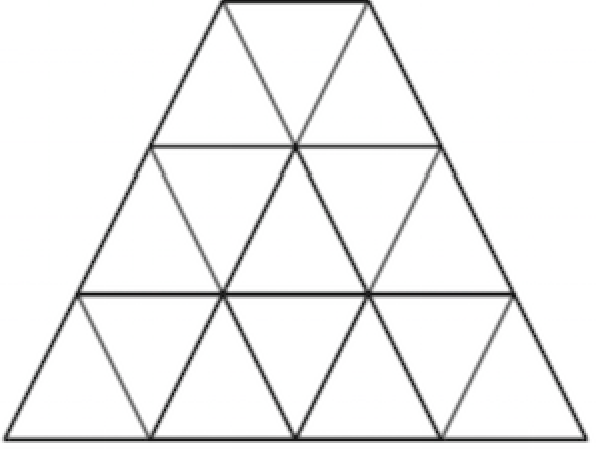
\includegraphics[ width=0.2\textwidth]{triangle.png}
\end{subfigure}
\caption{Structured instances: regular grid graph, regular grid graph with hole, regular triangular graph with cutting area }\label{fig2}
\end{figure}

\begin{figure}
\centering
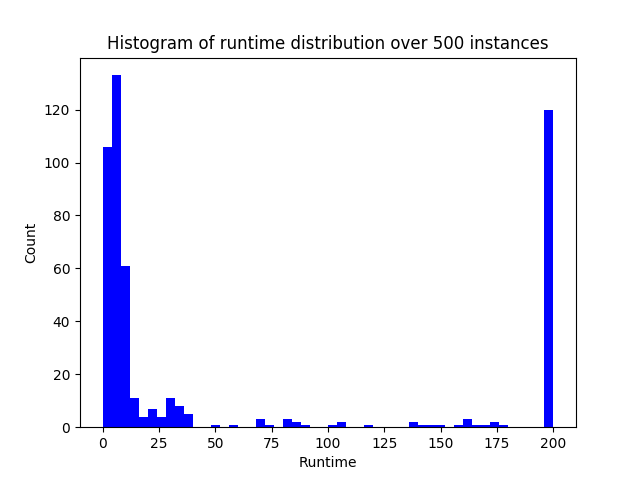
\includegraphics[width=0.7\textwidth]{hist10.png}
\caption{Runtime distribution of Encoding 2 on 500 different instances that are gained through eliminating random edges from a regular square grid graph with length of its side 10.}
\label{fig3}
\end{figure}

To use machine learning to construct a predictor of performance for a given 
instance of a particular encoding, we need informative and easy to compute 
instance features. In this work, we considered features of two types: graph
features and encoding-based features. Graph features either capture some
general characteristics of graphs such as the numbers of nodes and edges, the 
minimum and the maximum degrees, the minimum and maximum in- and out-degrees, 
etc., or reflect properties related to the problem at hand. Choosing 
problem-related graph features requires understanding of the problem domain. 
In our case, we selected for this group several features related to properties
of depth-first and breadth-first search trees rooted in the nodes of the graph
as they inform about reachability from a node. All graph features we used in 
our work are listed in Table \ref{graphfeatures} in Appendix B. 

Encoding-based features of an instance are obtained by grounding one or more 
encodings on an instance, and using the program 
\emph{claspre}.\footnote{https://potassco.org/labs/claspre/}
\emph{Claspre} is a light-weight version of the ASP solver 
\textit{clasp}\footnote{\url{https://potassco.org}} specialized for 
preprocessing. It extracts \emph{static} and \emph{dynamic} 
features of ground ASP programs while solving them for a short amount of time.
Static features of ground ASP programs are parameters of the program itself
such as the number of variables, rules and constraints (cf. 
Table~\ref{staticfeatures} in Appendix B). Dynamic features 
(cf. Table ~\ref{dynamicfeatures} in Appendix B) 
provide information about
the solving process. We are not using them in our work and so we do not 
discuss them any further.
%such as the number of choices, conflicts and learned 
%conflicts~\cite{cdcllearnt} at first two restarts of 
%the conflict-driven-clause-learning~\cite{cdcl1,cdcl2} 
solving procedure. In order to obtain claspre features of a graph 
instance, we combine the instance with our six encodings and then pass them 
to \textit{claspre}. 
%Table~\ref{tab0} gives a summary of features and feature 
%groups generated for our experiments. 
In total, there are 319 %569
features in 7%13 
groups, one gropup of graph features and six groups of \textit{claspre}
static %and dynamic claspre
features, one group for each encoding. This set is just a starting point for feature selection.
We narrow it down to avoid overfitting by identifying features that are
informative for the HC problem (we discuss this process in the next section).

%\begin{table}[]
%\caption{Summary of features and feature groups} \label{tab0}
%\programmath
%\begin{tabular}{c|c|c|c|c}
%\hline\hline
%instance & graph features (41) & claspre + encoding1 (88)&  ... & claspre + encoding6 (88) \\ 
                                % 
%\hline\hline
%\end{tabular}
%\programmath
%\end{table}

\section{Encoding Selection with Machine Learning}

The goal of encoding selection is to identify for a given instance encodings
that promise good performance. To learn performance models based on performance 
data one can use regression or classification. The former constructs regression 
models predicting each algorithm's performance expressed as the (predicted) 
running time. The latter builds multi-class machine learning models to directly 
select the most promising encoding from a collection of candidate encodings. 
Our work so far suggests that the regression approach works better than the 
classification one. Thus, from now on we concentrate on the former.

Our work is based on the performance data and instance features computed and
collected for the data set of 784 hard instances (as described above). We use 
this data to build regression models for the six encodings we constructed as 
representations of the HC problem. Specifically, we build $k$-nearest neighbor
(KNN), decision tree (DT) and random forest (RF) regressors. All these models 
are directly imported from python \emph{scikit-learn} package. Since the 
performance of machine learning methods depends on the hyper-parameter setting, 
we list below the hyper-parameters we choose for these models.
\begin{itemize}
\item The $k$-nearest neighbors predicts the value based on the average of $k$
nearest points under the pre-determined distance metric. The hyper-parameters 
of the $k$-nearest neighbors are the number $k$ of neighbors and the distance
metric. 
\item The decision tree is constructed top-down, with the training data 
divided by axis-parallel splits into different rectangular regions where 
the averages are used for prediction. The splits are determined by highest 
standard deviation reduction based on the decrease in standard deviation after
the dataset is split on attributes. The hyper-parameters are the maximum depth
of the tree, the minimum number of samples still to split, and the minimum 
number of samples in a leaf node. 
\item The random forest is created from an ensemble of decision trees that 
bootstrap various sub-samples of the original dataset, fit a tree for each, 
and use averaging to make predictions. The random forest can improve predictive 
accuracy and help control overfitting. Bootstrap is used in our decision-tree models. When bootstrap is used, the data for the 
sub-samples are drawn from the original dataset with replacement and all
sub-samples are of the same size. The random forest method has hyper-parameters 
concerning constituent decision trees and, in addition, the number of trees in 
a forest. 
\end{itemize} 

To select informative features from all the features computed we perform 
in-group individual feature selection followed by the feature group 
selection. To perform in-group individual feature selection for a group
of features, we start with an empty feature set, randomly add one or more 
features, and then test the average performance of selected features in 
terms of evaluation metrics(cf. Section \ref{metrics}) to decide whether to 
keep them or not. Next, we select feature groups by treating each feature 
group as a unit and attempting to add them one by one using the same method
as for the in-group selection.

To evaluate a particular set of selectd features, we randomly divide our data 
into the training set (80\%) and the test set (20\%), train models using the
training set, and test the performance of encoding selection result on the
test set. During the training process, we use the grid search to select proper 
hyper-parameters. First we define a list of values or a range for each 
hyper-parameter, and then select points from each range to train a specific
machine learning model. We build a model for each combination of
hyper-parameter values, evaluate the performance of the models, and select 
the architecture that performs best. Models are not directly trained on 
training set; instead, we use the 10-fold cross validation to improve the 
generalization performance. Given the training set, we partition it into ten 
disjoint bins $X_i$,~i $\in \{1,..,10\}$. For each $i=1,\ldots, 10$, we train
a model on the training set $X \setminus X_i$ and evaluate it on the validation 
set $X_i$. We then average the results. The grid search requires exhaustive 
sampling of all combinations of hyper-parameters so it increases the training 
time. 

The approach we described in this section resulted in a set of 42 features
(cf. Table~\ref{ecfeatures}), 27 graph features and 15 claspre static 
features. Our result shows that clapsre dynamic features are not as informative as graph features and claspre static features. However, since we performed the greedy feature selection method manually, it is very likely that we missed some features or feature groups that are more important to make predictions.

\begin{table}[]
\caption{Selected instance features for encoding selection} \label{ecfeatures}                                           
\programmath
	\begin{tabular}{lll}
		\hline\hline
ratio\_node\_edge                 & avg\_depth\_beam              & Frac\_Binary\_Rules\_hc2          \\
ratio\_bi\_edge                   & dfs\_1st\_back\_depth         & Frac\_Ternary\_Rules\_hc2         \\
avg\_out\_degree                  & sum\_of\_choices\_along\_path & Free\_Problem\_Variables\_hc2     \\
avg\_in\_degree                   & depth\_avg\_dfs\_backjump.    & Problem\_Variables\_hc2           \\
ratio\_of\_odd\_out\_degree       & depth\_back\_to\_root         & Assigned\_Problem\_Variables\_hc2 \\
ratio\_of\_even\_out\_degree      & depth\_back\_to\_any          & Constraints\_hc2                  \\
ratio\_of\_odd\_in\_degree        & depth\_one\_path              & Rules\_hc2                        \\
ratio\_of\_even\_in\_degree       & min\_depth\_bfs               & Frac\_Normal\_Rules\_hc2          \\
ratio\_of\_odd\_degree            & max\_depth\_bfs               & Frac\_Cardinality\_Rules\_hc2     \\
ratio\_of\_even\_degree           & avg\_depth\_bfs               & Frac\_Choice\_Rules\_hc2          \\
ratio\_out\_degree\_less\_than\_3 & min\_depth\_beam              & Frac\_Weight\_Rules\_hc2          \\
ratio\_in\_degree\_less\_than\_3  & max\_depth\_beam              & Frac\_Binary\_Constraints\_hc2    \\
ratio\_degree\_less\_than\_3      & avg\_depth\_beam              & Frac\_Ternary\_Constraints\_hc2   \\
avg\_depth\_bfs                   & Frac\_Unary\_Rules\_hc2      & Frac\_Other\_Constraints\_hc2  \\
\hline\hline
	\end{tabular}
\programmath
\end{table}

\section{Experimentation}

\subsection{Hardware and evaluation metrics }\label{metrics}
Our experiments were conducted on a computer with four cores, each with
Intel i7-7700 3.60GHz CPU and 16GB RAM, running under 64-bit 18.04.2 LTS 
(Bionic Beaver) Ubuntu system. The solver used is 
\emph{clasp}\footnote{https://potassco.org} version
3.3.2 with default parameter setting. The grounding tool 
is \emph{gringo}\footnote{https://potassco.org} version 4.5.4. We choose 
200 CPU seconds as 
cutoff time. All runs that exceed the cutoff time were terminated and penalized 
with the corresponding runtime (as explained above).

To evaluate the effectiveness of encoding selection, we compare the percentage 
of solved instances by the encoding selection method, by individual encodings,
and by the ``oracle'' method always correctly predicting the best perfroming 
encoding for an instance. We use the running time as a secondary measure.

%In the following, we present the results of encoding selection experiments 
%we have performed on the HC problem. Table \ref{tab8} shows the performance of 
%each encoding as well as the oracle performance on the test set.

\subsection{Performance on the test set}

The performance of individual encodings and of the oracle-based encoding
selection method are summarized in Table~\ref{testsetperf}. For each encoding,
it lists the percentage of solved instances from the test set (the \emph{solved
percentage}), the average solved runtime and the number of times that encoding 
had the smallest runtime (was the ``winner''). We use the solved percentage 
as the primary evaluation metric, and the average runtime as the secondary 
one. The test set contains 156 instances randomly selected from the original 
data set of 780. The best individual encoding, Encoding 1, solves 131 or 
84.0\% of test instances. However, among these 131 solved instances, 
Encoding 1 is the fastest one only 21 times and it also has the highest 
average running time (due to relatively frequent timeouts). Encoding 4 is 
the fastest the largest number of times (37) but it only solves 78.8\% 
of instances (ranks third in this measure). Overall, the results show that 
the encodings we used in the experiment have complementary strengths, with 
each of them being the best one with some frequency.

The last line in the table presents the oracle-based encoding selection
performance (always select and run the best encoding for an instance). It 
solves 98.7\%, or 154 out of 156 instances, with the average runtime of 
21.1. Compared with Encoding 1, the best of the six encodings, the 
always-select-best selection method solves 14.7\% more instances. 
We note that 98.7\% is the upper bound for the performance that could 
be achieved by encoding selection. It indicates to the potential for an 
intelligent encoding selection method to outperform individual encodings.

\begin{table}
	\caption{The performance of individual encodings and of the 
oracle selection on test set} \label{testsetperf}
	\programmath
	\begin{tabular}{llll}
		\hline\hline
		%
		& Solved Percentage\% & Average Solved Runtime & Number of 
Wins\\ \hline%
		Single encoding performance & & &                                     \\ %
		Encoding 1        & 84.0          & 82.4                      & 21            \\ %
		Encoding 2        & 71.2           & 44.0                      & 31            \\ %
		Encoding 3        & 56.4           & 30.7                       & 33            \\ %
		Encoding 4        & 78.8           & 38.6                      & 37            \\ %
		Encoding 5        & 57.1          & 35.4                      & 19            \\ %
		Encoding 6        & 79.5          & 48.1                      & 15            \\\hline %
		Oracle performance  & & &                                               \\ %
		Oracle            & 98.7           & 21.1                      &               \\ \hline\hline
	\end{tabular}
	\programmath
\end{table}

\subsection{Analysis of encoding selection results}

We performed encoding selection experiments using different machine learning 
methods on the training set and test set described earlier. The models were
trained with the narrowed down set of features and hyper-parameters set to
values obtained in the hyper-parameter tuning process, as discussed above).
The results are shown in Table~\ref{ecresult1}. 

Our best predictor based on the decision tree method, solves 96.2\% of 
instances, or 150 out of 156. This is very close to 98.7\% of solved
instances for the always-select-best oracle. Even the worst performing of 
three machine learning models, based on the $k$-nearest neighbors algorithm,
solves 92.9\% of instances, much better than any individual encoding. We 
also note that the second best model, the RF predictor, solves 146 out of 
156 instances, only four instances fewer than the DT predictor. Overall, we 
find taht each of the three machine learning methods we studied provide 
promising results in terms of the percentage of the solved instances. However, 
the average runtimes for solved instances of these machine learning methods 
are much higher than the reunning time of 21.1s for the oracle. The reason 
is that sometimes the performance prediction models select the second best
encoding rather than the best one.

\begin{table}
\caption{Test result of encoding selection experiment } \label{ecresult1}
\programmath
\begin{tabular}{llll}
\hline\hline
%
                  & Solved Percentage\% & Average Solved Runtime & Number of Wins \\ \hline%
Single encoding performance & & &                                     \\ %
Encoding 1        & 84.0           & 82.4                      & 25            \\ %
Encoding 2        & 71.2           & 44.0                      & 29            \\ %
Encoding 3        & 56.4           & 30.7                       & 20            \\ %
Encoding 4        & 78.8           & 38.6                      & 28            \\ %
Encoding 5        & 57.1           & 35.4                      & 26            \\ %
Encoding 6        & 79.4           & 48.1                      & 26            \\\hline %
Oracle performance  & & &                                               \\ %
Oracle            & 98.7           & 21.1                      &               \\ \hline
Encoding selection & & &                                                \\ %
Encoding selection (KNN) & 92.9          & 40.2                    &               \\ %
Encoding selection (DT) & 96.2&42.2       &               \\ %
Encoding selection (RF) & 93.6&41.7	      &               \\ %
\hline\hline
\end{tabular}
\programmath
\end{table}

In order to test the effectiveness of the proposed encoding selection method, 
we repeated our experiment using a different random partition of the data set 
into the training and test sets. The results are shown in Table~\ref{ecresult2}.
The results are similar to those of the first experiment. All machine learning 
methods result in performance improvement over any single encodings. The 
encoding selection method with random forest models improves the performance 
of the single best encoding, Encoding 6, by 13.5\% in terms of solved 
percentage, solving 21 more instances out of the total 156. At the same time, 
we find that the average solved runtimes of these encoding selection methods 
are still higher than that of the oracle. In difference to the previous results,
the best machine learning method in this experiment is the random forest but 
the decision-tree predictor is a very close second. 
%We analyze the results of the random forest model and the decision tree model 
%for both experiments and find that the performance of these two models are so 
%close that we can not conclude which model is better for our method. 

\begin{table}[]
	\caption{Test result of (2nd) encoding selection experiment} \label{ecresult2}
	\programmath
	\begin{tabular}{llll}
		\hline\hline
		%
		& Solved Percentage\% & Average Solved Runtime & Number of Wins \\ \hline%
		Single encoding performance & & &                                     \\ %
		Encoding 1        & 81.4&86.7                      & 18            \\ %
		Encoding 2        & 75.0 & 49.7                      & 24            \\ %
		Encoding 3        & 59.0&30.5                       & 17            \\ %
		Encoding 4        & 76.9&40.0                      & 35            \\ %
		Encoding 5        & 56.4&25.7                      & 30            \\ %
		Encoding 6        & 82.7&51.0                      & 32            \\\hline %
		Oracle performance  & & &                                               \\ %
		Oracle            & 100.0           & 21.8                      &               \\ \hline
		Encoding selection & & &                                                \\ %
		Encoding selection (KNN) & 91.7&45.2                    &               \\ %
		Encoding selection (DT) & 94.2&39.1      &               \\ %
		Encoding selection (RF) & 96.2&45.6	      &               \\ %
		\hline\hline
	\end{tabular}
	\programmath
\end{table}


\section{Summary}
We applied machine learning techniques to build performance prediction models
for different encodings of the HC problem. To this ends, we constructed
six encodings of the HC problem that showed complementary strengths on our 
data set. We designed a set of features characterizing problem instances (some
of them problem independent, and some reflecting features of the problem of 
interest). Finally, we applied three kinds of regression models to construct 
performance predictors. We used these predictors for to select an encoding 
for an instance before running an ASP solver. 

We tested the performance of different machine learning regression models and 
found that our encoding selection method yielded promising prediction results.
After running encoding selection to solve the HC problem for instances in our 
test sets, we observed our approach solved more instances than any individual 
encoding did coming close to the performance level of the oracle. We conclude 
that the encoding selection method is effective in improving the solving
capabilitis of ASP solvers.


\section{Future Work}

It is unsatisfactory that the running time of our encoding selection approach 
is higher (about two times higher in our experiments) than the optimal time of 
the always-select-best oracle. Closing that gap is a challenge that will 
require more accurate runtime prediction. One way to attack the problem is
to identify more informative features, especially domain-specific features
--- in our case, those capturing properties of graphs that are correlated 
with existence (or non-existence) of Hamiltonian cycles. Also, as is all known, feature selection can remove irrelevant and redundant attributes and has huge impacts on the performance of machine learning models. Through generating more useful domain-specific features and selecting more relevant features, we can obtain more promising results.

Another factor that affects the performance of solving an ASP problem is a 
specific solver used to perform the search. State-of-the-art solvers come 
with tens or even hundreds of parameters whose setting controls the search
process. The default parameter configuration may be good overall but more 
often than not will not be optimal on specific instances. Work on parameter
configuration, such as ParamILS~\cite{HutterHLS09}, has shown that a 
well-chosen parameter configuration can help achieve a performance improvement 
of over one order of magnitude. In our experiment, we used the default version 
of clasp. Our next step is to combine encoding selection with parameter 
configuration. 

The encoding candidates in our experiments were created and modified manually. 
We generated several encoding based on different representing ideas and rewrote 
them into their equivalent forms. However, it is desirable to automate the 
process, that is, to generate candidates with a tool that is able to analyze 
an encoding and rewrite it into several equivalent and efficient forms. 

\section*{Acknowledgements}
This work was funded by the NSF under the grant IIS-1707371.

\bibliography{refs2}

\newpage
\section*{Appendix A: Encodings}
We describe below the six encodings of the HC problems used in our 
experiments. %All of our encodings use the notion of reachability from
%node 1 as specified in Figure \ref{reachencod2}.\footnote{The constraint 
%requiring every node is reachable from every other node, as in Figure 
%\ref{reachencod}, has a larger grounding size and is in general inferior.}
%They differ only in the way we select edges and constrain the numbers of
%selected edges that leave and enter a node. Therefore, the figures below 
%list only the rules in the ``select-edges'' block for each encoding. 

\begin{figure}[!h]
\figrule
\begin{center}
\begin{verbatim}
%Generator
{ hcyc(X,Y) : link(X,Y) }:-node(X).
{ hcyc(X,Y) : link(X,Y) }:-node(Y).

:- 2{ hcyc(X,Y) : link(X,Y) },node(X).
:- 2{ hcyc(X,Y) : link(X,Y) },node(Y).

:- { hcyc(X,Y) : link(X,Y) }0,node(X).
:- { hcyc(X,Y) : link(X,Y) }0,node(Y).

%rule
reach(1).
reach(Y) :- reach(X),hcyc(X,Y).

%test
:- not reach(X),node(X).

%show
#show hcyc/2.
\end{verbatim}
\end{center}
\figrule
\caption{Hamiltonian Cycle Encoding 1}\label{enc1}
\end{figure}
\begin{figure}[!h]
\figrule
\begin{center}
\begin{verbatim}
%Generator
{ hcyc(X,Y) : link(X,Y) } =1:-node(X).
{ hcyc(X,Y) : link(X,Y) } =1:-node(Y).

%rule
reach(X) :- hcyc(1,X).
reach(Y) :- reach(X),hcyc(X,Y).

%test
:- not reach(X),node(X).

%show
#show hcyc/2.
\end{verbatim}
\end{center}
\figrule
\caption{Hamiltonian Cycle Encoding 2}\label{enc2}
\end{figure}

\begin{figure}[!h]
\figrule
\begin{center}
\begin{verbatim}
%Generator
{ hcyc(X,Y) : link(X,Y) } 1:-node(X).
{ hcyc(X,Y) : link(X,Y) } 1:-node(Y).

%rule
reach(X) :- hcyc(1,X).
reach(Y) :- reach(X),hcyc(X,Y).

%test
:- not reach(X),node(X).

%show
#show hcyc/2.


\end{verbatim}
\end{center}
\figrule
\caption{Hamiltonian Cycle Encoding 3}\label{enc3}
\end{figure}

\begin{figure}[!h]
\figrule
\begin{center}
\begin{verbatim}
%Generator
{ hcyc(X,Y) : link(X,Y) } :-node(X).
{ hcyc(X,Y) : link(X,Y) } :-node(Y).

:- 2{ hcyc(X,Y) : link(X,Y) },node(X).
:- 2{ hcyc(X,Y) : link(X,Y) },node(Y).

:- { hcyc(X,Y) : link(X,Y) }0,node(X).
:- { hcyc(X,Y) : link(X,Y) }0,node(Y).

%rule
reach(X) :- hcyc(1,X).
reach(Y) :- reach(X),hcyc(X,Y).

%test
:- not reach(X),node(X).

%show
#show hcyc/2.

\end{verbatim}
\end{center}
\figrule
\caption{Hamiltonian Cycle Encoding 4}\label{enc4}
\end{figure}

\begin{figure}[!h]
\figrule
\begin{center}
\begin{verbatim}
%Generator
{ hcyc(X,Y) : link(X,Y) } :-node(X).
{ hcyc(X,Y) : link(X,Y) } :-node(Y).

:- 2{ hcyc(X,Y) : link(X,Y) },node(X).
:- 2{ hcyc(X,Y) : link(X,Y) },node(Y).

%rule
reach(X) :- hcyc(1,X).
reach(Y) :- reach(X),hcyc(X,Y).

%test
:- not reach(X),node(X).

%show
#show hcyc/2.
\end{verbatim}
\end{center}
\figrule
\caption{Hamiltonian Cycle Encoding 5}\label{enc5}
\end{figure}

\begin{figure}[!h]
\figrule
\begin{center}
\begin{verbatim}
%Generator
{ hcyc(X,Y) : link(X,Y) }  =1:-node(X).
{ hcyc(X,Y) : link(X,Y) }  =1:-node(Y).

%rule
reach(1).
reach(Y) :- reach(X),hcyc(X,Y).

%test
:- not reach(X),node(X).

%show
#show hcyc/2.
\end{verbatim}
\end{center}
\figrule
\caption{Hamiltonian Cycle Encoding 6}\label{enc6}
\end{figure}

\newpage
\section*{Appendix B: Instance Features}\label{appB}

We considered the following 41 graph features and, as explained earlier, 
selected 27 of them to the set of features to be used by learning 
algorithms (cf. Table \ref{ecfeatures}).

%\begin{table}[!h]
%\caption{A list of graph features} \label{graphfeatures}
%\begin{tabular}{lll}
%num\_of\_nodes              & ratio\_of\_even\_out\_degree      & ratio\_degree\_less\_than\_3  \\
%num\_of\_edges              & num\_of\_odd\_in\_degree          & depth\_dfs\_1st\_backjump        \\
%ratio\_node\_edge           & ratio\_of\_odd\_in\_degree        & sum\_of\_choices\_along\_path \\
%bi\_edge                    & num\_of\_even\_in\_degree         & depth\_avg\_dfs\_backjump     \\
%ratio\_bi\_edge             & ratio\_of\_even\_in\_degree       & depth\_back\_to\_root         \\
%min\_out\_degree            & num\_of\_odd\_degree              & depth\_back\_to\_any          \\
%max\_out\_degree            & ratio\_of\_odd\_degree            & depth\_one\_path              \\
%avg\_out\_degree            & num\_of\_even\_degree             & min\_depth\_bfs               \\
%min\_in\_degree             & ratio\_of\_even\_degree           & max\_depth\_bfs               \\
%max\_in\_degree             & out\_degree\_less\_than\_3        & avg\_depth\_bfs               \\
%avg\_in\_degree             & ratio\_out\_degree\_less\_than\_3 & min\_depth\_beam              \\
%num\_of\_odd\_out\_degree   & in\_degree\_less\_than\_3         & max\_depth\_beam              \\
%ratio\_of\_odd\_out\_degree & ratio\_in\_degree\_less\_than\_3  & avg\_depth\_beam              \\
%num\_of\_even\_out\_degree  & degree\_less\_than\_3             &                              
%\end{tabular}
%\end{table}

\begin{description}
\item[num\_of\_nodes:] the number of nodes in a graph
\item[ratio\_node\_edge:] the number of edges in a grpah
\item[ratio\_node\_edge:] the ratio of the number of node to the edge
\item[bi\_edge:] the number of bidirected edges
\item[ratio\_bi\_edge:] the ratio of bidirected edges over all edges
\item[min\_out\_degree:] the mininum of outdegree of nodes
\item[max\_out\_degree:] the maxinum of outdegree of nodes
\item[avg\_out\_degree:] the average of outdegree of nodes
\item[min\_in\_degree:] the mininum of indegree of nodes
\item[max\_in\_degree:] the maxinum of indegree of nodes
\item[avg\_in\_degree:] the average of indegree of nodes
\item[num\_of\_odd\_out\_degree:] the number of nodes with odd outdegree
\item[ratio\_of\_odd\_out\_degree:] the ratio of the number of nodes with odd outdegree over the total nodes
\item[num\_of\_even\_out\_degree:] the number of nodes with even outdegree
\item[ratio\_of\_even\_out\_degree:] the ratio of the number of nodes with even outdegree over the total nodes
\item[num\_of\_odd\_in\_degree:] the number of nodes with odd indegree
\item[ratio\_of\_odd\_in\_degree:] the ratio of the number of nodes with odd indegree over the total nodes
\item[num\_of\_even\_in\_degree:] the number of nodes with even indegree
\item[ratio\_of\_even\_in\_degree:] the ratio of the number of nodes with even indegree over the total nodes
\item[num\_of\_odd\_degree:] the number of nodes with odd degree (in+out)
\item[ratio\_of\_odd\_degree:] the ratio of the number of nodes with odd degree (in+out) over all nodes
\item[num\_of\_even\_degree:] the number of nodes with even degree (in+out)
\item[ratio\_of\_even\_degree:] the ratio of the number of nodes with even degree (in+out) over all nodes
\item[out\_degree\_less\_than\_3:] the number of nodes with outdegree less than 3
\item[ratio\_out\_degree\_less\_than\_3:] the ratio of the number of nodes with outdegree less than 3 over all nodes
\item[in\_degree\_less\_than\_3:] the number of nodes with indegree less than 3
\item[ratio\_in\_degree\_less\_than\_3:] the ratio of the number of nodes with indegree less than 3 over all nodes
\item[degree\_less\_than\_3:] the number of nodes with degree(in+out) less than 3
\item[ratio\_degree\_less\_than\_3:] the ratio of the number of nodes with degree(in+out) less than 3 over all nodes
\item[depth\_dfs\_1st\_backjump:] Run DFS from node 1, return the depth of first backjump, where the algorithm discovers no new nodes
\item[sum\_of\_choices\_along\_path:] When depth\_dfs\_1st\_backjump, return the total number of choices of each discovered nodes along the DFS path
\item[depth\_avg\_dfs\_backjump:] Run DFS from node 1, return the average depth of all backjumps defined above
\item[depth\_back\_to\_root:] Run DFS from node 1, return the depth of a node that has back edge to node 1
\item[depth\_back\_to\_any:] Run DFS from node 1, return the depth of a node that has back edge to any discoverd node
\item[depth\_one\_path:] Run DFS from node 1, return the depth of first node with only one path, or one child
\item[min\_depth\_bfs:] Run BFS from node 1, record the depth of all the dead nodes, the node with no new nodes attached to it, and return the minimum
\item[max\_depth\_bfs:] Run BFS from node 1, record the depth of all the dead nodes and return the maxinum
\item[avg\_depth\_bfs:] Run BFS from node 1, record the depth of all the dead nodes and return the average
\item[min\_depth\_beam:] Run beam search, a two branches BFS search, from node 1, record the depth of all the dead nodes, the node with no new nodes attached to it, and return the minimum
\item[max\_depth\_beam:] Run beam search from node 1, record the depth of all the dead nodes and return the maxinum
\item[avg\_depth\_beam:] Run beam search from node 1, record the depth of all the dead nodes and return the average
\end{description}

We also considered features extracted by running \textit{claspre} on each of 
the six encodings. As a result, there are six groups of static and dynamic 
features shown in Tables \ref{staticfeatures} and \ref{dynamicfeatures},
respectively, one for each encoding. Features in each group for Encoding 
$i$, $i=1,2,\ldots,6$, are denoted by the \textit{claspre} name appended 
with the identifier of an encoding (for instance, Frac\_Neg\_Body\_hc3). We 
refer to \textit{claspre}\footnote{\url{https://potassco.org/labs/claspre/}}
for more information about these features. We recall that our feature selection process resulted in 15 \textit{claspre} features selected for the set of 
features we used in modeling, all of them obtained from running \textit{claspre}
on Encoding 2, and all of them static (cf. Table \ref{ecfeatures}).


\begin{table}[!h]
\caption{A list of claspre static features} \label{staticfeatures}
\ \\
\begin{tabular}{lll}
Frac\_Neg\_Body              & Program\_Atoms            & Atom-Atom\_Equivalences       \\
Frac\_Pos\_Body              & SCCS                      & Body-Body\_Equivalences       \\
Frac\_Unary\_Rules           & Nodes\_in\_Positive\_BADG & Other\_Equivalences           \\
Frac\_Binary\_Rules          & Rules                     & Frac\_Atom-Atom\_Equivalences \\
Frac\_Ternary\_Rules         & Normal\_Rules             & Frac\_Body-Body\_Equivalences \\
Frac\_Integrity\_Rules       & Cardinality\_Rules        & Frac\_Other\_Equivalences     \\
Tight                        & Choice\_Rules             & Binary\_Constraints           \\
Problem\_Variables           & Weight\_Rules             & Ternary\_Constraints          \\
Free\_Problem\_Variables     & Frac\_Normal\_Rules       & Other\_Constraints            \\
Assigned\_Problem\_Variables & Frac\_Cardinality\_Rules  & Frac\_Binary\_Constraints     \\
Constraints                  & Frac\_Choice\_Rules       & Frac\_Ternary\_Constraints    \\
Constraints/Vars             & Frac\_Weight\_Rules       & Frac\_Other\_Constraints      \\
Created\_Bodies              & Equivalences              &                              
\end{tabular}
\end{table}

\begin{table}[!h]
\caption{A list of claspre dynamic features of one restart} \label{dynamicfeatures}
\ \\
\begin{tabular}{lll}
Choices                         & Literals\_in\_Loop\_Nogoods           & Frac\_Learnt\_Ternary                    \\
Conflicts/Choices               & Frac\_Literals\_in\_Conflict\_Nogoods & Frac\_Learnt\_Others                     \\
Avg\_Conflict\_Levels           & Frac\_Literals\_in\_Loop\_Nogoods     & Skipped\_Levels\_while\_Backjumping      \\
Avg\_LBD\_Levels                & Removed\_Nogoods                      & Avg\_Skipped\_Levels\_while\_Backjumping \\
Learnt\_from\_Conflict          & Learnt\_Binary                        & Longest\_Backjumping                     \\
Learnt\_from\_Loop              & Learnt\_Ternary                       & Running\_Avg\_Conflictlevel              \\
Frac\_Learnt\_from\_Conflict    & Learnt\_Others                        & Running\_Avg\_LBD                        \\
Frac\_Learnt\_from\_Loop        & Frac\_Removed\_Nogood                 &                                          \\
Literals\_in\_Conflict\_Nogoods & Frac\_Learnt\_Binary                  &                                         
\end{tabular}
\end{table}

\end{document}
\begin{thebibliography}{}


\bibitem[\protect\citeauthoryear{Eiter and Gottlob and Mannila}{Eiter and Gottlob and Mannila}{1997}]{eiterasp}
{\sc Eiter, T. and Gottlob, G. and Mannila, H} 1997.
\newblock Disjunctive Datalog.
\newblock ACM TODS 22(3):364–418

\bibitem[\protect\citeauthoryear{Marek and Truszczynski}{Marek and Truszczynski}{1998}]{mmasp}
{\sc Victor W. Marek and Mirek Truszczynski} 1998.
\newblock Stable Models and an Alternative Logic Programming Paradigm.
\newblock CoRR cs.LO/9809032.


\bibitem[\protect\citeauthoryear{Holger and Marius and Torsten}{Holger and Marius and Torsten}{2014}]{holger:claspfolio}
  {\sc Holger Hoos and Marius Lindauer and Torsten Schaub3} 2014.
  \newblock claspfolio 2: Advances in Algorithm Selection for Answer Set Programming.
  \newblock Theory and Practice of Logic Programming


\bibitem[\protect\citeauthoryear{Carla and John}{Carla and John}{2001}]{algportfolio}
{\sc Carla P. Gomes and Bart Selman} 2001.
\newblock Algorithm portfolios.
\newblock Artificial Intelligence, v.126 n.1-2, p.43-62.

\bibitem[\protect\citeauthoryear{John. R. Rice}{John. R. Rice}{1975}]{rice:as}
  {\sc John. R. Rice} 1975.
  \newblock The Algorithm Selection Problem.
  \newblock Advances in Computers. Vol 15.

\bibitem[\protect\citeauthoryear{M. Maratea, etc.}{M. Maratea, etc.}{2011}]{measp}
  {\sc Marco Maratea and Luca Pulina and Francesco Ricca} 2011.
  \newblock ME-ASP: A Multi-Engine Solver for Answer Set
Programming
  \newblock LPNMR 2011: Logic Programming and Nonmonotonic Reasoning pp 352-357
 
 \bibitem[\protect\citeauthoryear{Lin Xu, etc.}{Lin Xu, etc.}{2008}]{satzilla}
  {\sc Lin Xu and Frank Hutter and Holger H. Hoos and Kevin Leyton-Brown} 2008.
  \newblock SATzilla: Portfolio-based Algorithm Selection for SAT.
  \newblock Journal of Artificial Intelligence Research 32 (2008) 565-606.
  
  
\bibitem[\protect\citeauthoryear{F. Hutter, etc.}{F. Hutter, etc.}{2009}]{frank:paramILS}
  {\sc Frank Hutter and Holger H. Hoos and Kevin Leyton-Brown} 2009.
  \newblock ParamILS: An Automatic Algorithm Configuration Framework.
  \newblock Journal of Artificial Intelligence Research. Vol 36. P267--306.

\bibitem[\protect\citeauthoryear{Gebser and Kaminski and Kaufmann and Ostrowski and Schaub and Thiele}{Gebser and Kaminski and Kaufmann and Ostrowski and Schaub and Thiele}{2009}]{clasphelper}
{\sc Gebser and Kaminski and Kaufmann and Ostrowski and Schaub and Thiele}
\newblock A user’s guide to gringo, clasp,
clingo, and iclingo
\newblock https://sourceforge.net/projects/potassco/files/guide/2.0/guide-2.0.pdf/


\bibitem[\protect\citeauthoryear{Potassco}{Potassco}{}]{claspre}
  {\sc Potassco} 
  \newblock claspre
  \newblock https://potassco.org/labs/claspre/
  

\bibitem[\protect\citeauthoryear{ }{ }{}]{sklearn}
{\sc } 
\newblock Scikit-learn
\newblock https://scikit-learn.org/

\bibitem[\protect\citeauthoryear{Gebser and Kaufmann and Neumann and Schaub}{Gebser and Kaufmann and Neumann and Schaub}{2007}]{clasppaper}
{\sc Martin Gebser and Benjamin Kaufmann and Andre Neumann and Torsten Schaub} 2007
\newblock Conflict-driven answer set solving
\newblock IJCAI’07, AAAI Press (2007) 386–392



\bibitem[\protect\citeauthoryear{Potassco}{Potassco}{}]{claspweb}
  {\sc Potassco}  
  \newblock clasp
  \newblock https://potassco.org/clasp/

\bibitem[\protect\citeauthoryear{Potassco}{Potassco}{}]{gringo}
{\sc Potassco} 
\newblock gringo
\newblock https://potassco.org/clingo/

\bibitem[\protect\citeauthoryear{M. Alviano}{M. Alviano}{2013}]{wasp}
{\sc M. Alviano and C. Dodaro and W. Faber and N. Leone, and Francesco Ricca}
\newblock  WASP: A Native ASP Solver Based on Constraint Learning. 
\newblock Proceedings of LPNMR (2013)
\bibitem[\protect\citeauthoryear{Gebser and Kaufmann and Neumann and Schaub}{Gebser and Kaufmann and Neumann and Schaub}{2007}]{cdcllearnt}
{\sc M. Gebser and B. Kaufmann and A. Neumann and T. Schaub} 
\newblock Conflict-driven answer set solving 
\newblock Proceedings of the Twentieth International Joint Conference
on Artificial Intelligence (IJCAI’07), pages 386–392. AAAI
Press/The MIT Press, 2007

\bibitem[\protect\citeauthoryear{Davis and Putnam}{Davis and Putnam}{1960}]{cdcl1}
{\sc Martin Davis and Hillary Putnam} 1960
\newblock A computing procedure for quantification theory 
\newblock Journal of ACM, 7:201–215


\bibitem[\protect\citeauthoryear{Davis and Logemannand and Loveland and Schaub}{Davis and Logemannand and Loveland}{1962}]{cdcl2}
{\sc Martin Davis and George Logemannand and Donald Loveland} 1962
\newblock Conflict-driven answer set solving 
\newblock Communications of the ACM, 5(7):394–397


\bibitem[\protect\citeauthoryear{M. Nogueira, etc.}{M. Nogueira, etc.}{2001}]{nasa}
  {\sc Monica Nogueira and Marcello Balduccini and Michael Gelfond and Richard Watson and Matthew Barry} 2001.
  \newblock An A-prolog decision support system for the space shuttle.
  \newblock Practical Aspects of Declarative Languages pp 169-183.
  
\bibitem[\protect\citeauthoryear{Georg Boenn, etc.}{Georg Boenn, etc.}{2008}]{music}
  {\sc Georg Boenn and Martin Brain and Marina De Vos and John ffitch} 2008.
  \newblock Automatic Composition of Melodic and Harmonic Music by Answer Set Programming.
  \newblock Logic Programming pp 160-174
  
 
\bibitem[\protect\citeauthoryear{E. Erdem and F. Ture}{E. Erdem and F. Ture}{2008}]{haplo}
  {\sc Esra Erdem and Ferhan Ture} 2008
  \newblock Efficient Haplotype Inference with Answer Set Programming
  \newblock Proceedings of the Twenty-third National Conference on Artificial Intelligence (AAAI08), pp 436-441.
  

\bibitem[\protect\citeauthoryear{C. Dodaro and M. Maratea}{C. Dodaro and M. Maratea}{2017}]{nurse}
  {\sc Carmine Dodaro and Marco Maratea} 2017.
  \newblock Nurse scheduling via Answer Set Programming.
  \newblock Logic Programming and Nonmonotonic Reasoning pp 301-307
  
\end{thebibliography}

\label{lastpage}
\end{document}

% end of new_TLP2egui.tex
